\section{Incarnation 1}
  \begin{flushleft}
    The logic for computing Cos, Sin, Pi and other functions was written from the ground up in this incarnation. Code snippets are below.
  \end{flushleft}
  \subsection{Snippets}
  \vspace{2em}
    \begin{figure}[h!]
      \centering
      \frame{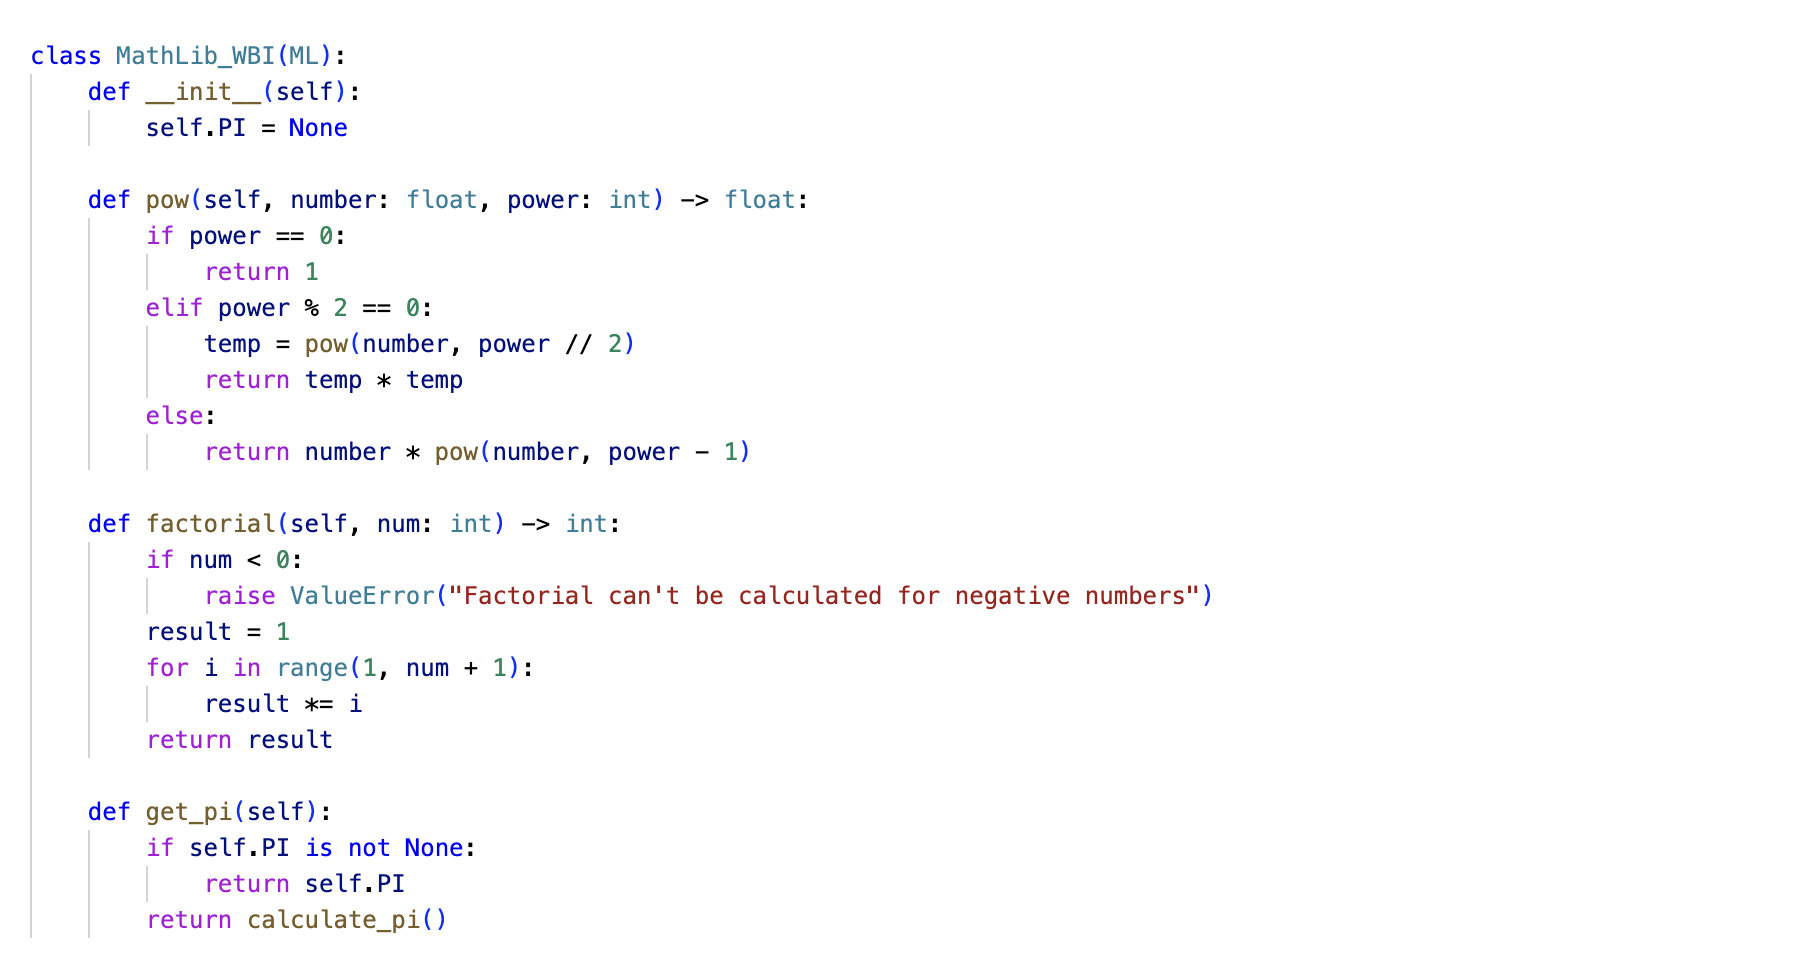
\includegraphics[scale= 0.4]{resources/snippets/MathWBI.png}}
      \caption{Logic to compute Exponent, Factorial and Pi}
      \label{fig:Math Library}
    \end{figure}
    \pagebreak
    \begin{figure}[h!]
      \centering
      \frame{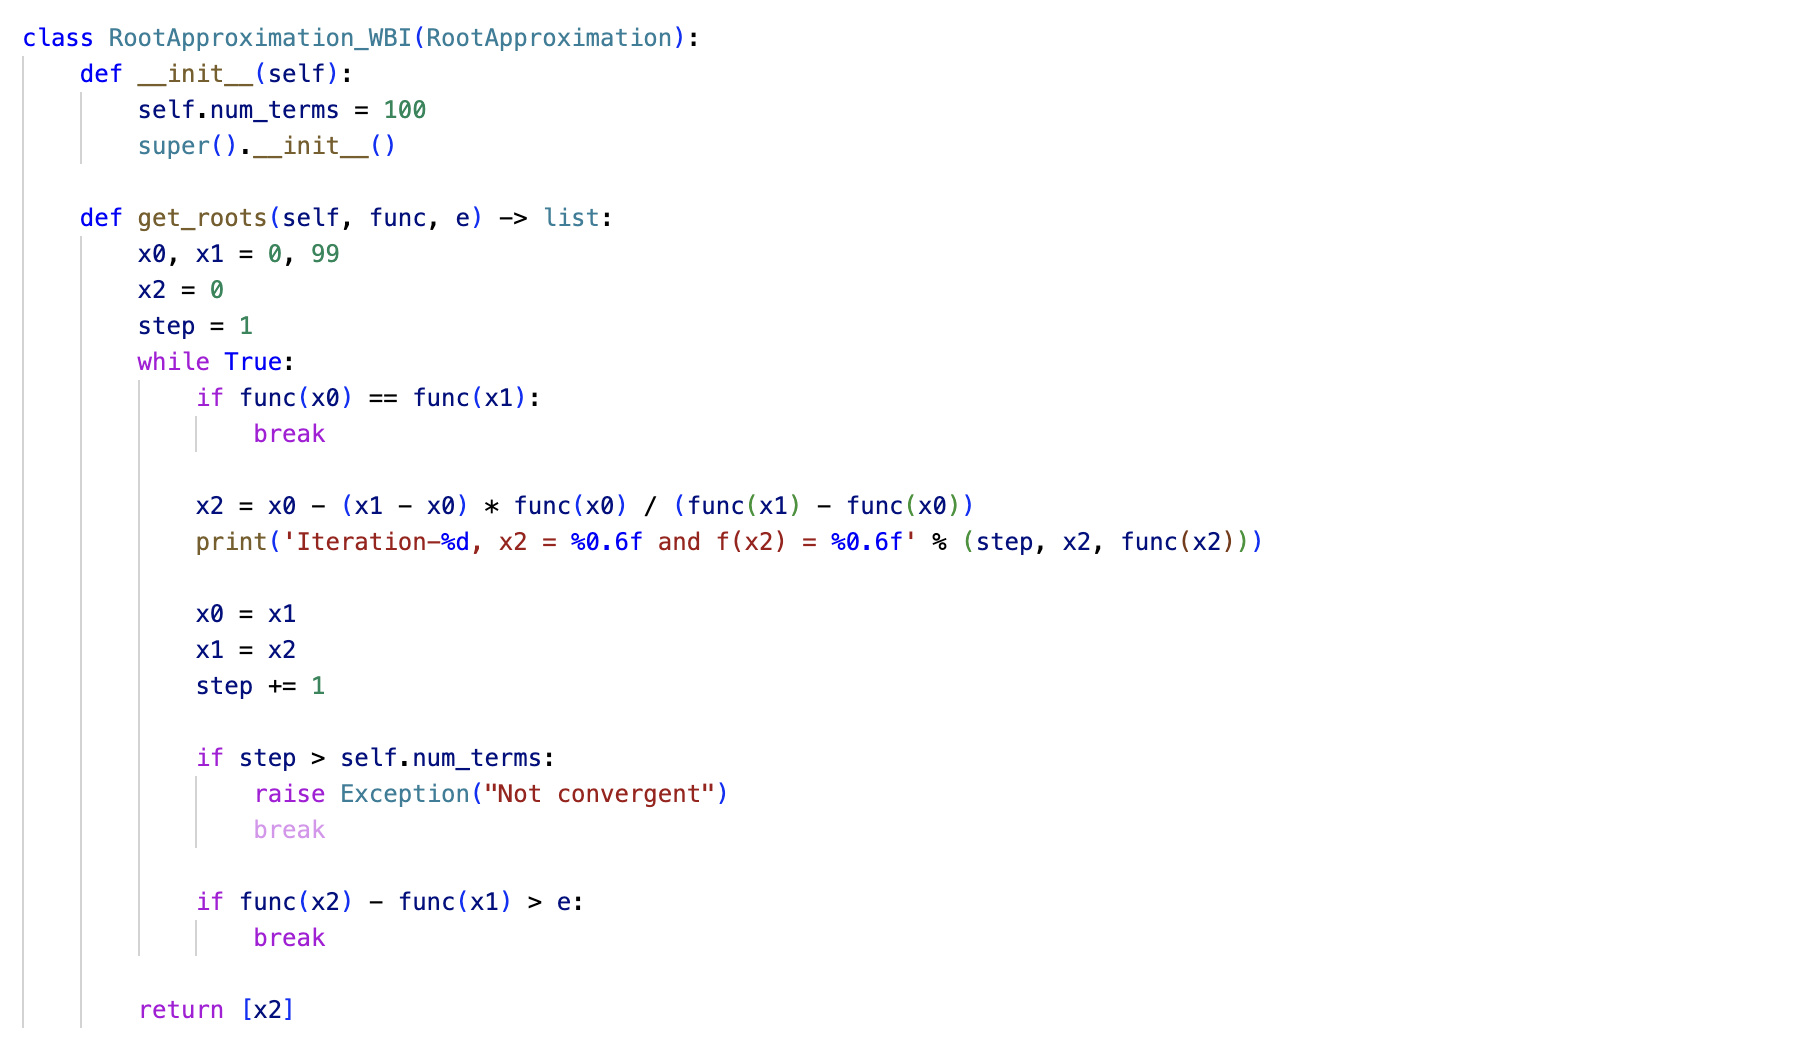
\includegraphics[scale= 0.4]{resources/snippets/RootApWBI.png}}
      \caption{Secant Method of root approximation}
      \label{fig:Root Approximation}
    \end{figure}

    \begin{figure}[h!]
      \centering
      \frame{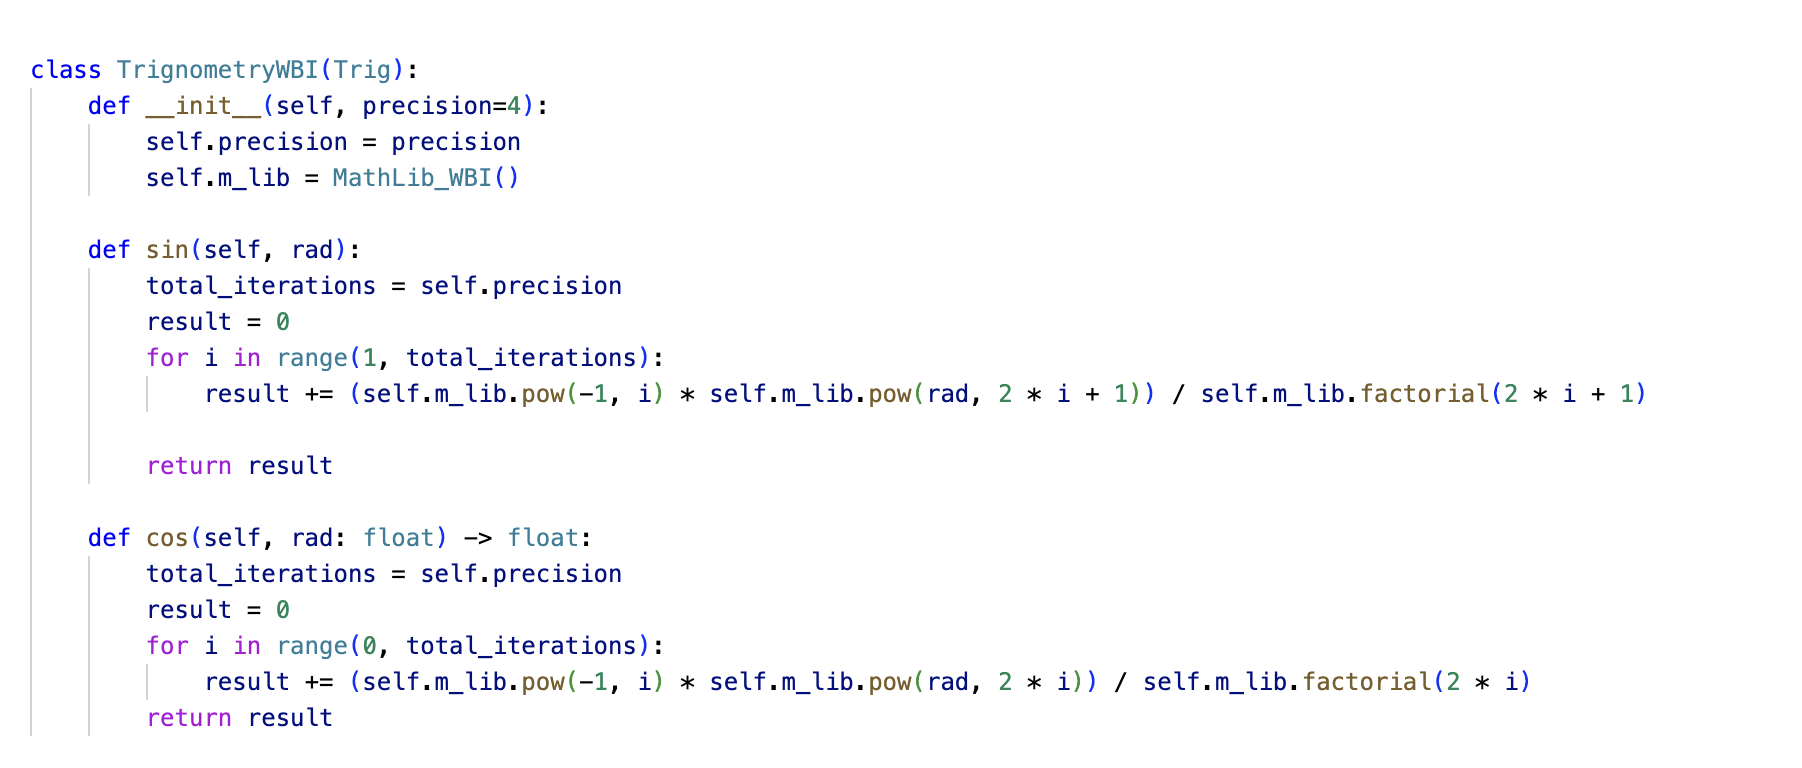
\includegraphics[scale= 0.4]{resources/snippets/TrigonometryWBI.png}}
      \caption{Logic to compute trigonometry functions}
      \label{fig:trigonometric Functions}
    \end{figure}
    \pagebreak

    \subsection{Output}
    \begin{figure}[h!]
      \centering
      \frame{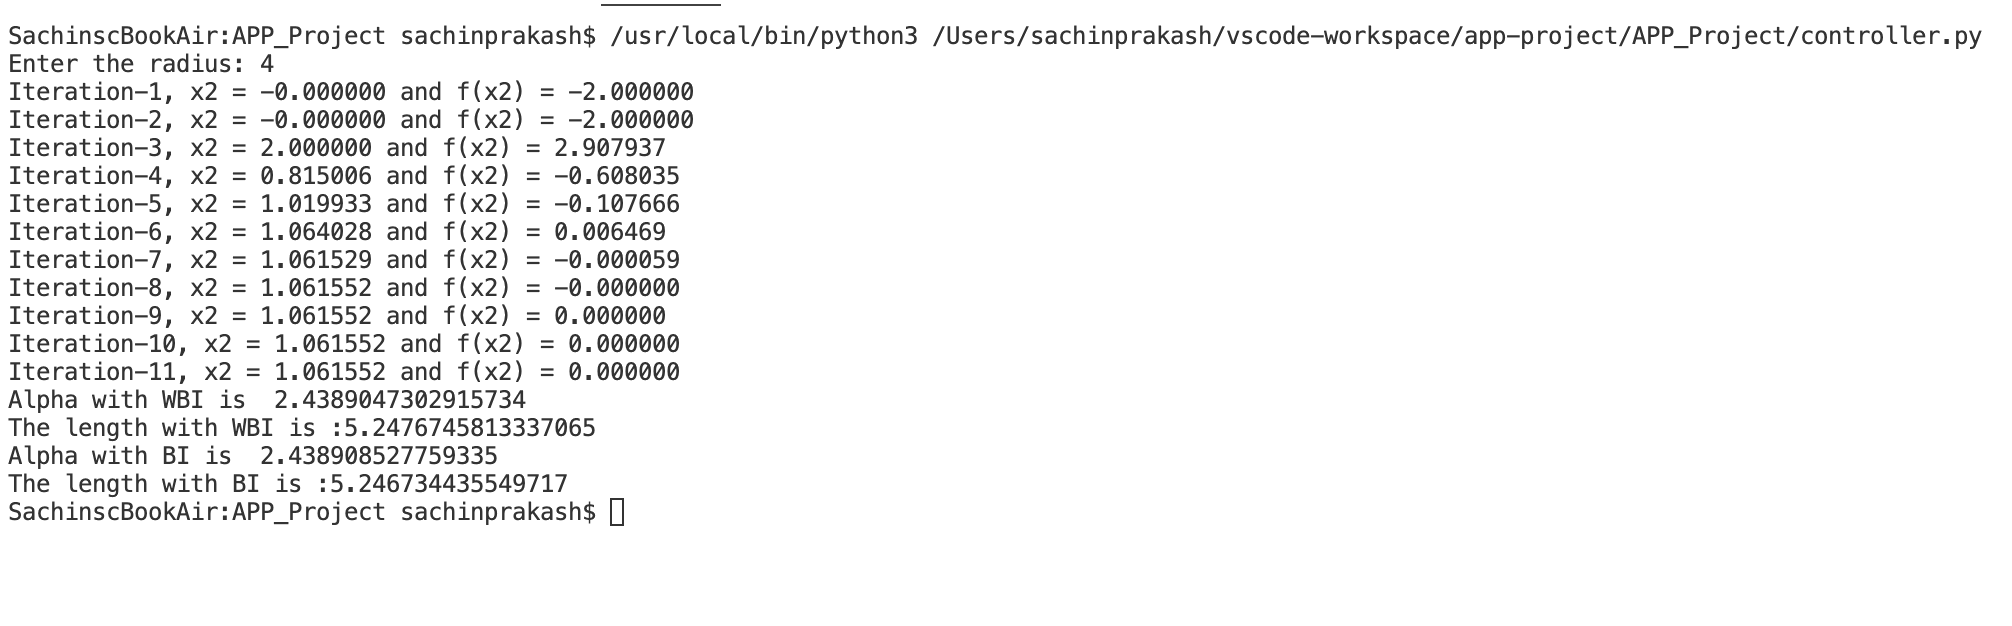
\includegraphics[scale= 0.4]{resources/snippets/inc1OP.png}}
      \caption{Output for Incarnation 1}
      \label{fig:Text-based output}
    \end{figure}
    \pagebreak

\section{Incarnation 2}
  \begin{flushleft}
    The python Math module and SciPy library were used to compute the various values. Code snippets are below.
  \end{flushleft}

  \subsection{Snippets}
  \vspace{2em}
    \begin{figure}[h!]
      \centering
      \frame{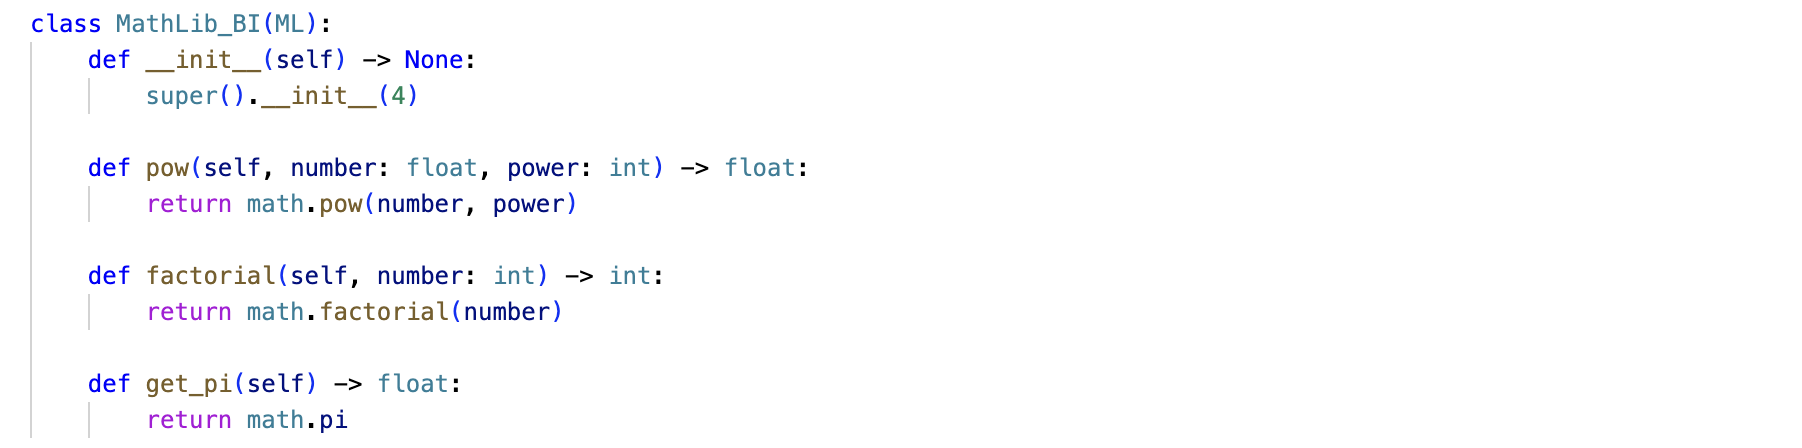
\includegraphics[scale= 0.4]{resources/snippets/MathBI.png}}
      \caption{Math module functions}
      \label{fig:Library functions for math}
    \end{figure}

    \begin{figure}[h!]
      \centering
      \frame{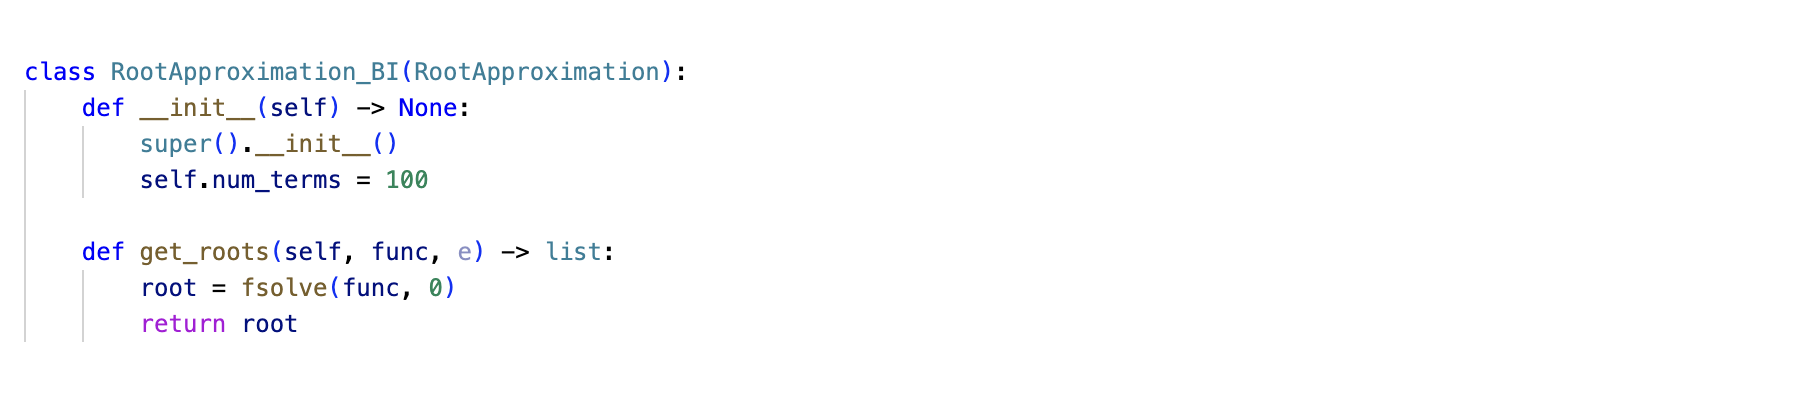
\includegraphics[scale= 0.4]{resources/snippets/RootApBI.png}}
      \caption{Root approximation using SciPy}
      \label{fig:SciPy Root Approximation}
    \end{figure}

    \begin{figure}[h!]
      \centering
      \frame{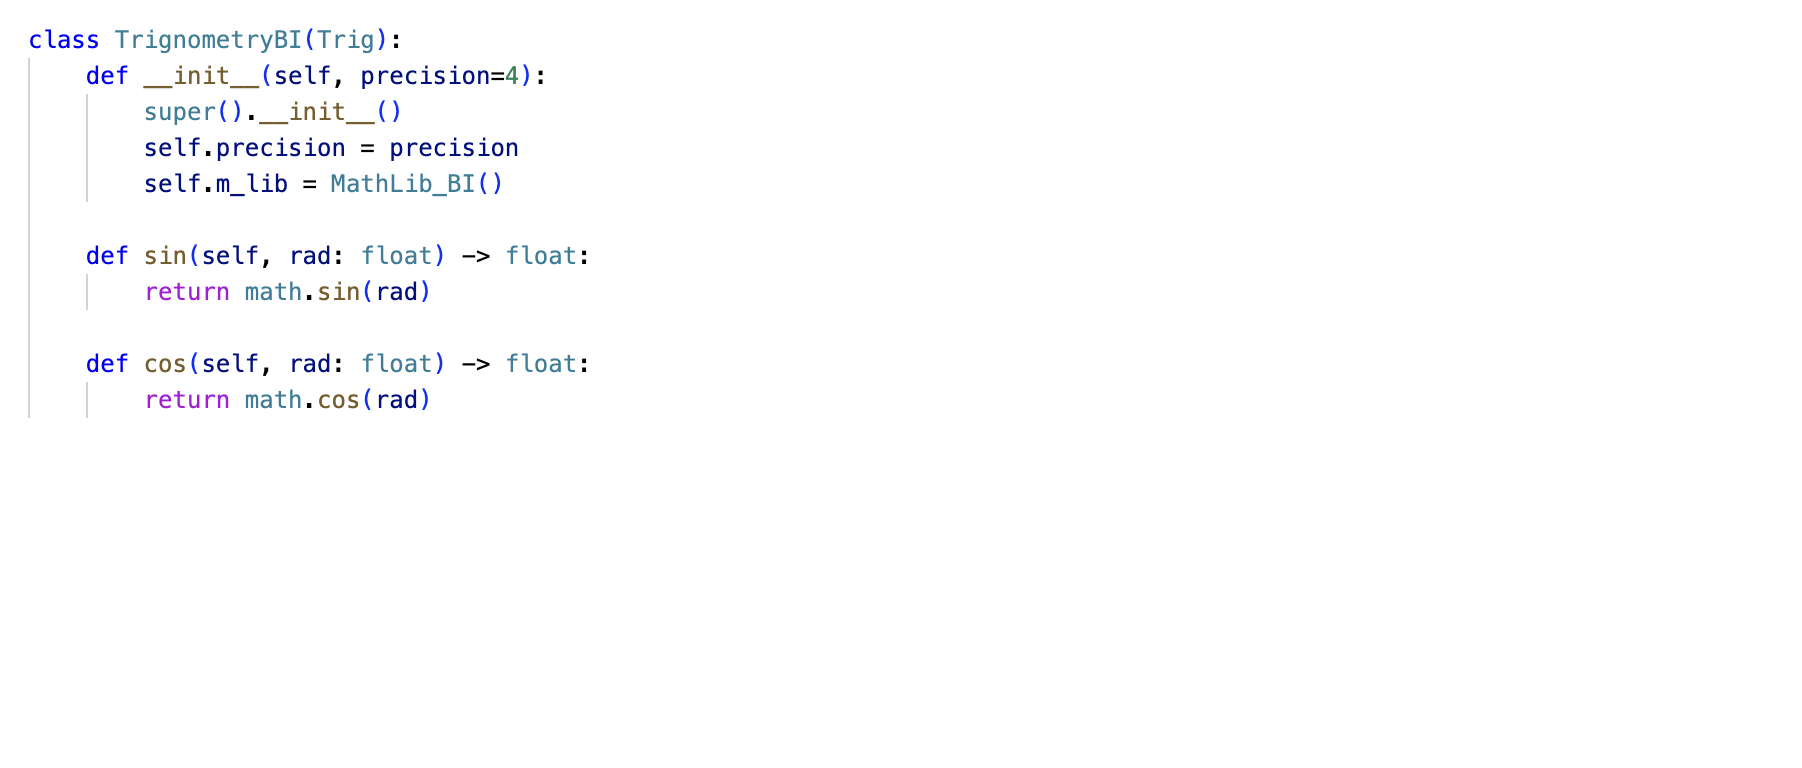
\includegraphics[scale= 0.4]{resources/snippets/TrigonometryBI.png}}
      \caption{Math module Trigonometry functions}
      \label{fig:Math trigonometry functions}
    \end{figure}
    \begin{figure}[h!]
      \centering
      \frame{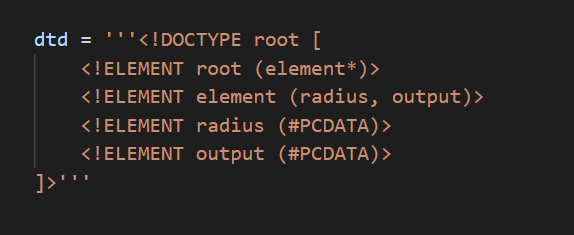
\includegraphics[scale= 1.0]{resources/dtd.png}}
      \caption{DTD of xml file}
      \label{fig:dtd of the output xml file}
    \end{figure}
    \subsection{Output}
    \begin{figure}[h!]
      \centering
      \frame{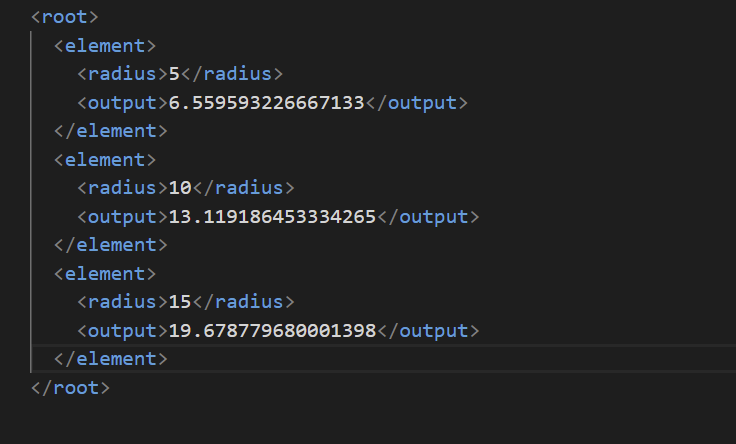
\includegraphics[scale= 0.8]{resources/outputxml.png}}
      \caption{XML file generated from user data}
      \label{fig:output xml file}
    \end{figure}
    \pagebreak

   

\addtocontents{toc}{\protect\setcounter{tocdepth}{1}}
\section{Quality Attributes}
  \begin{flushleft}
    The following attributes apply to both incarnations.
  \end{flushleft}
  \subsection{Modifiability}
    \begin{flushleft}
      Modifiability refers to the efforts that will be needed to modify the software product according to the specific requirements of customers\cite{8343604}. The source code was built using the RDD paradigm. This inherently makes it amenable to updates in the future.
    \end{flushleft}

  \subsection{Readability}
    \begin{flushleft}
      Adequate comments were provided to make the source code more meaningful to the reader. The variable and method names adhere to the guidelines provided under PEP 8. 
    \end{flushleft}

  \subsection{Reusability}
    \begin{flushleft}
      The source code was made reusable by following the Single Responsibility Principle (SRP) for every class and method. Abstract types have been used to hide the implementation details and improve the composability.
    \end{flushleft}

  \subsection{Understandability}
    \begin{flushleft}
      The understandability of the source code was improved through
      \begin{itemize}
        \item {The use of meaningful variable names}
        \item {Inclusion of method and class descriptions}
        \item {Minimizing the complexity within each method in a class}
      \end{itemize}
    \end{flushleft}

  \subsection{Testability}
    \begin{flushleft}
      Due to the object-oriented nature of the project design, each class and method in the source code can be unit tested. Each class has its own set of tests which can swiftly determine if the actual value matches the expected.
    \end{flushleft}

  \subsection{Robustness}
  \begin{flushleft}
    All possible exceptions have been handled throughout the program and the potential points of failure have been minimized. In case of an exceptional event, a meaningful error message will be returned to the end user.
  \end{flushleft}

  \subsection{Generality}
    \begin{flushleft}
      The program has been made more general by avoiding the use of OS-specific path(s). E.g. When writing to an output file, a relative path name was used.
    \end{flushleft}

    \subsection{Usability}
    \begin{flushleft}
      The usability of the program has been improved by 
      \begin{itemize}
        \item {Using meaningful prompt messages throughout the lifecycle }
        \item {Minimizing the potential points of failure }
        \item {Returning meaningful error messages in case of an exceptional event}
      \end{itemize}
    \end{flushleft}
  
  \section{Version Control}
    The project was executed on GitHub with each of the team members working on the agreed-upon tasks. The final build of the project was achieved by merging the efforts from all team members.
    
    \begin{figure}[h!]
      \centering
      \frame{\href{https://github.com/ns-saini/APP_Project}{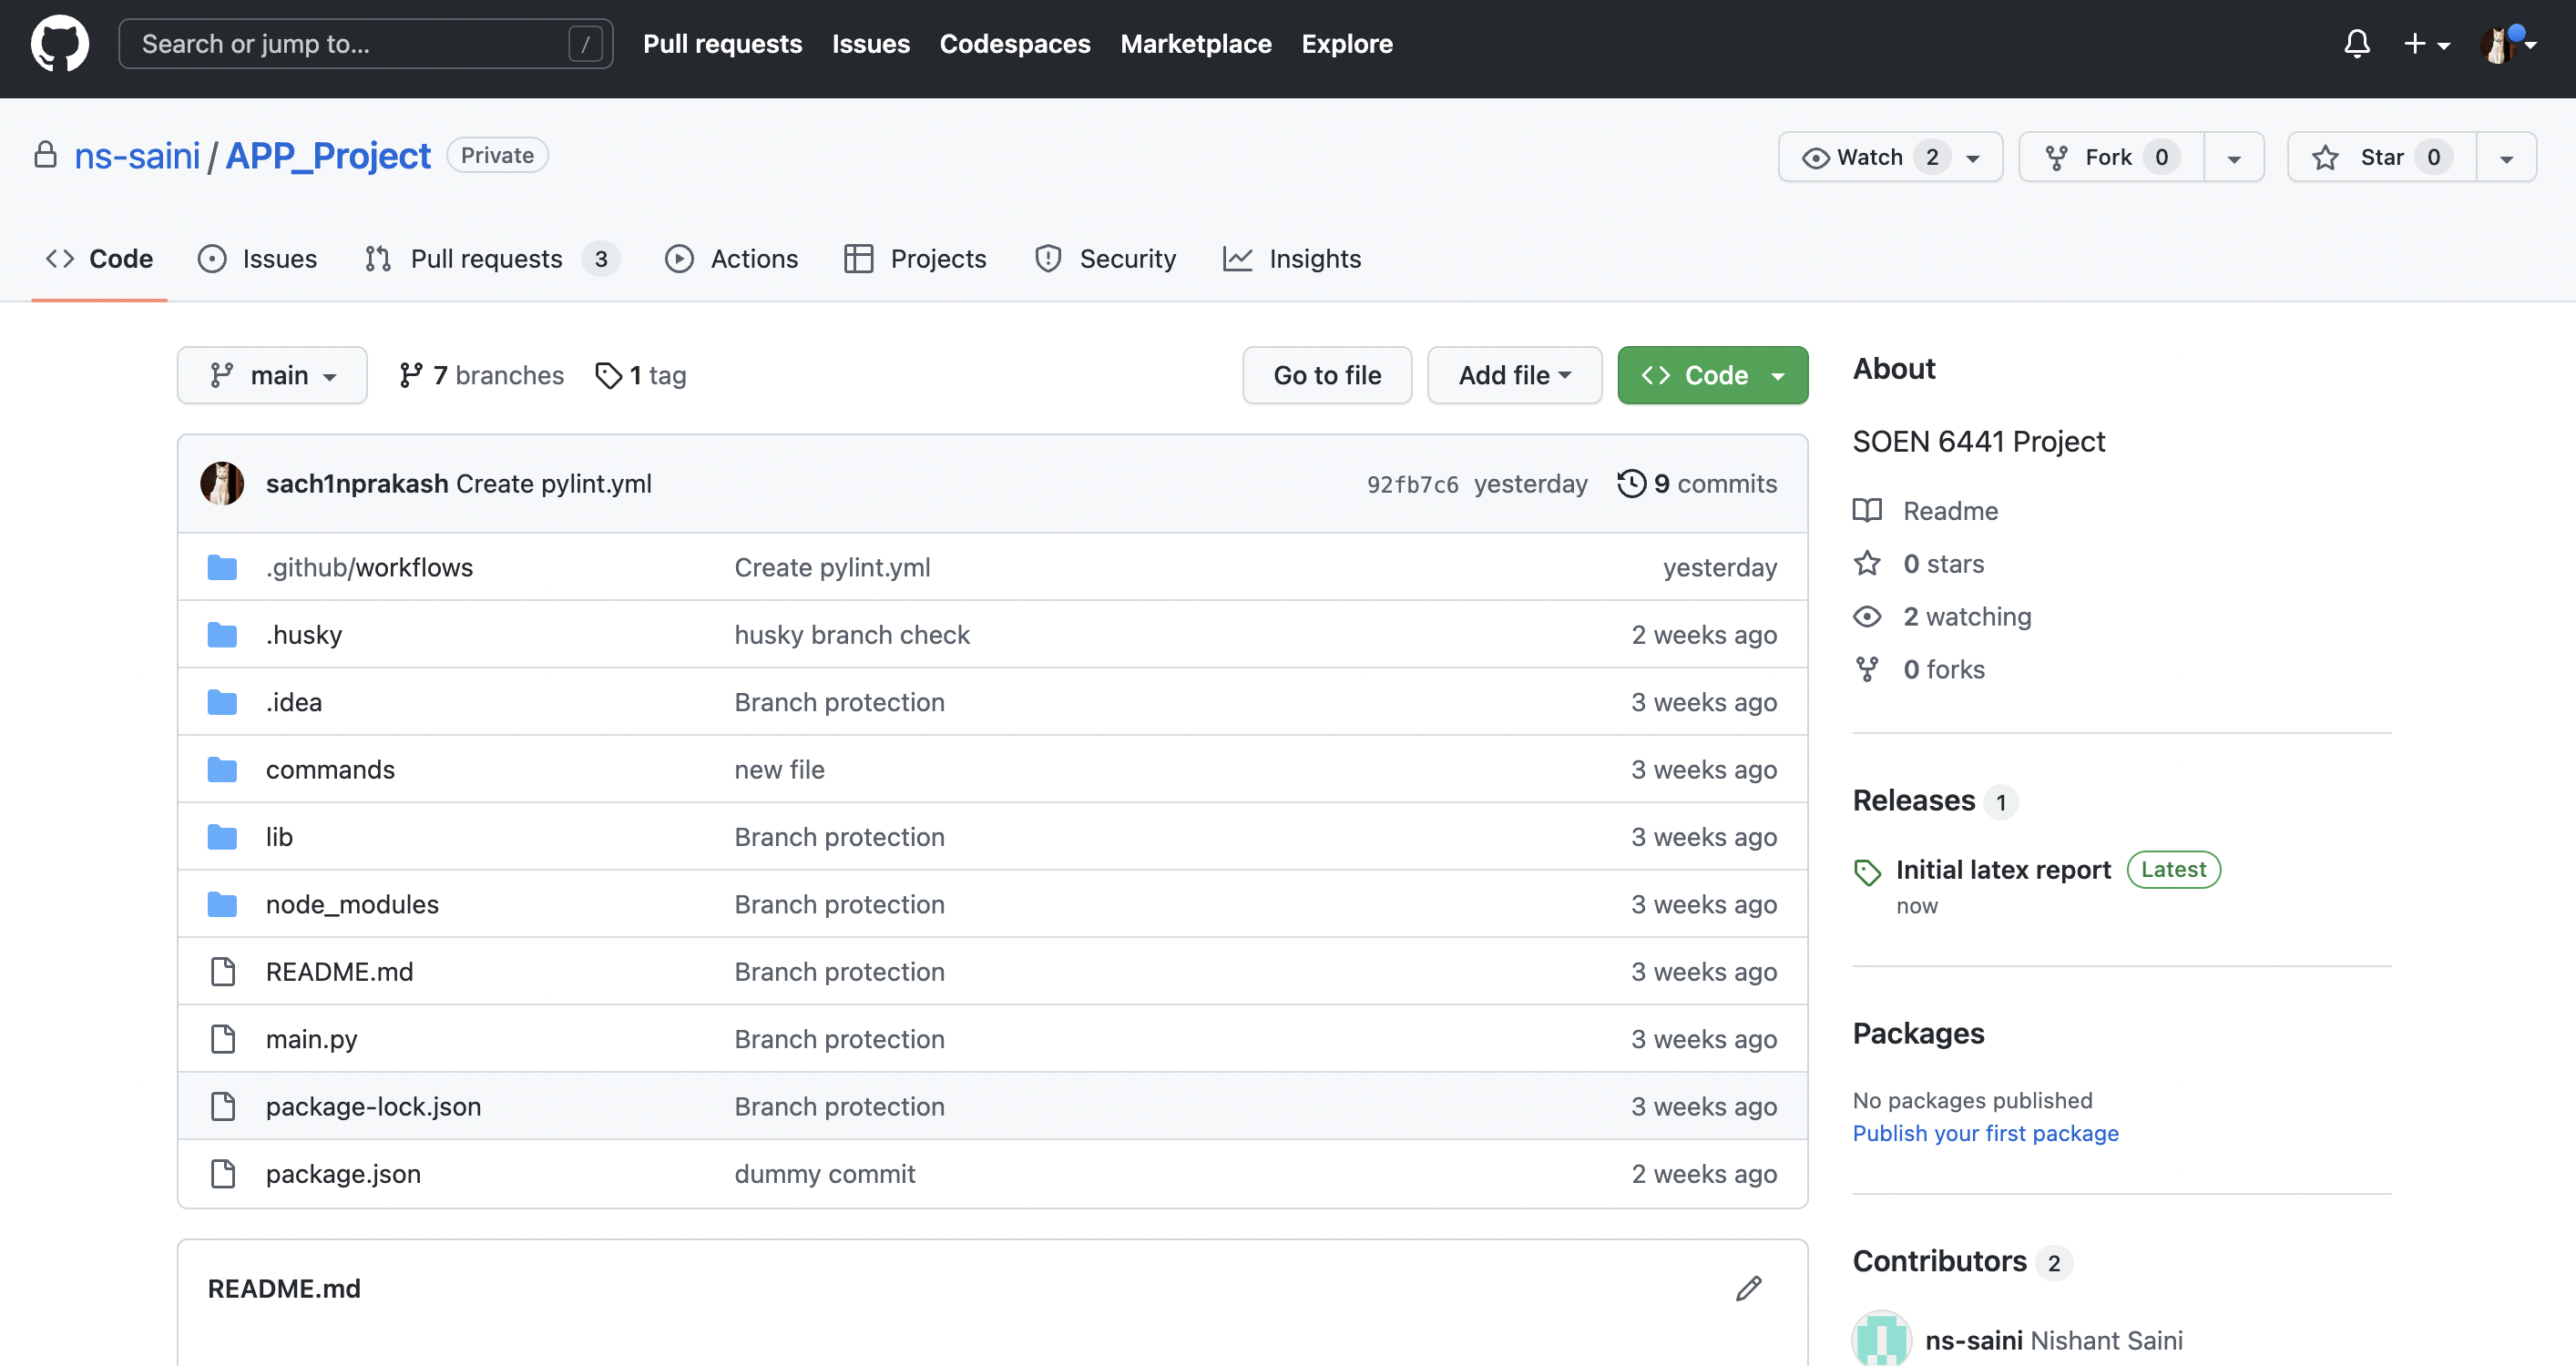
\includegraphics[scale= 0.3]{resources/github.png}}}
      \caption{\url{https://github.com/ns-saini/APP_Project}}
      \label{fig:Repository}
    \end{figure}

  \pagebreak
  \section{Debugger}
    The python debugger built into vs code was used during the development of the source code.
    \begin{figure}[h!]
      \centering
      \frame{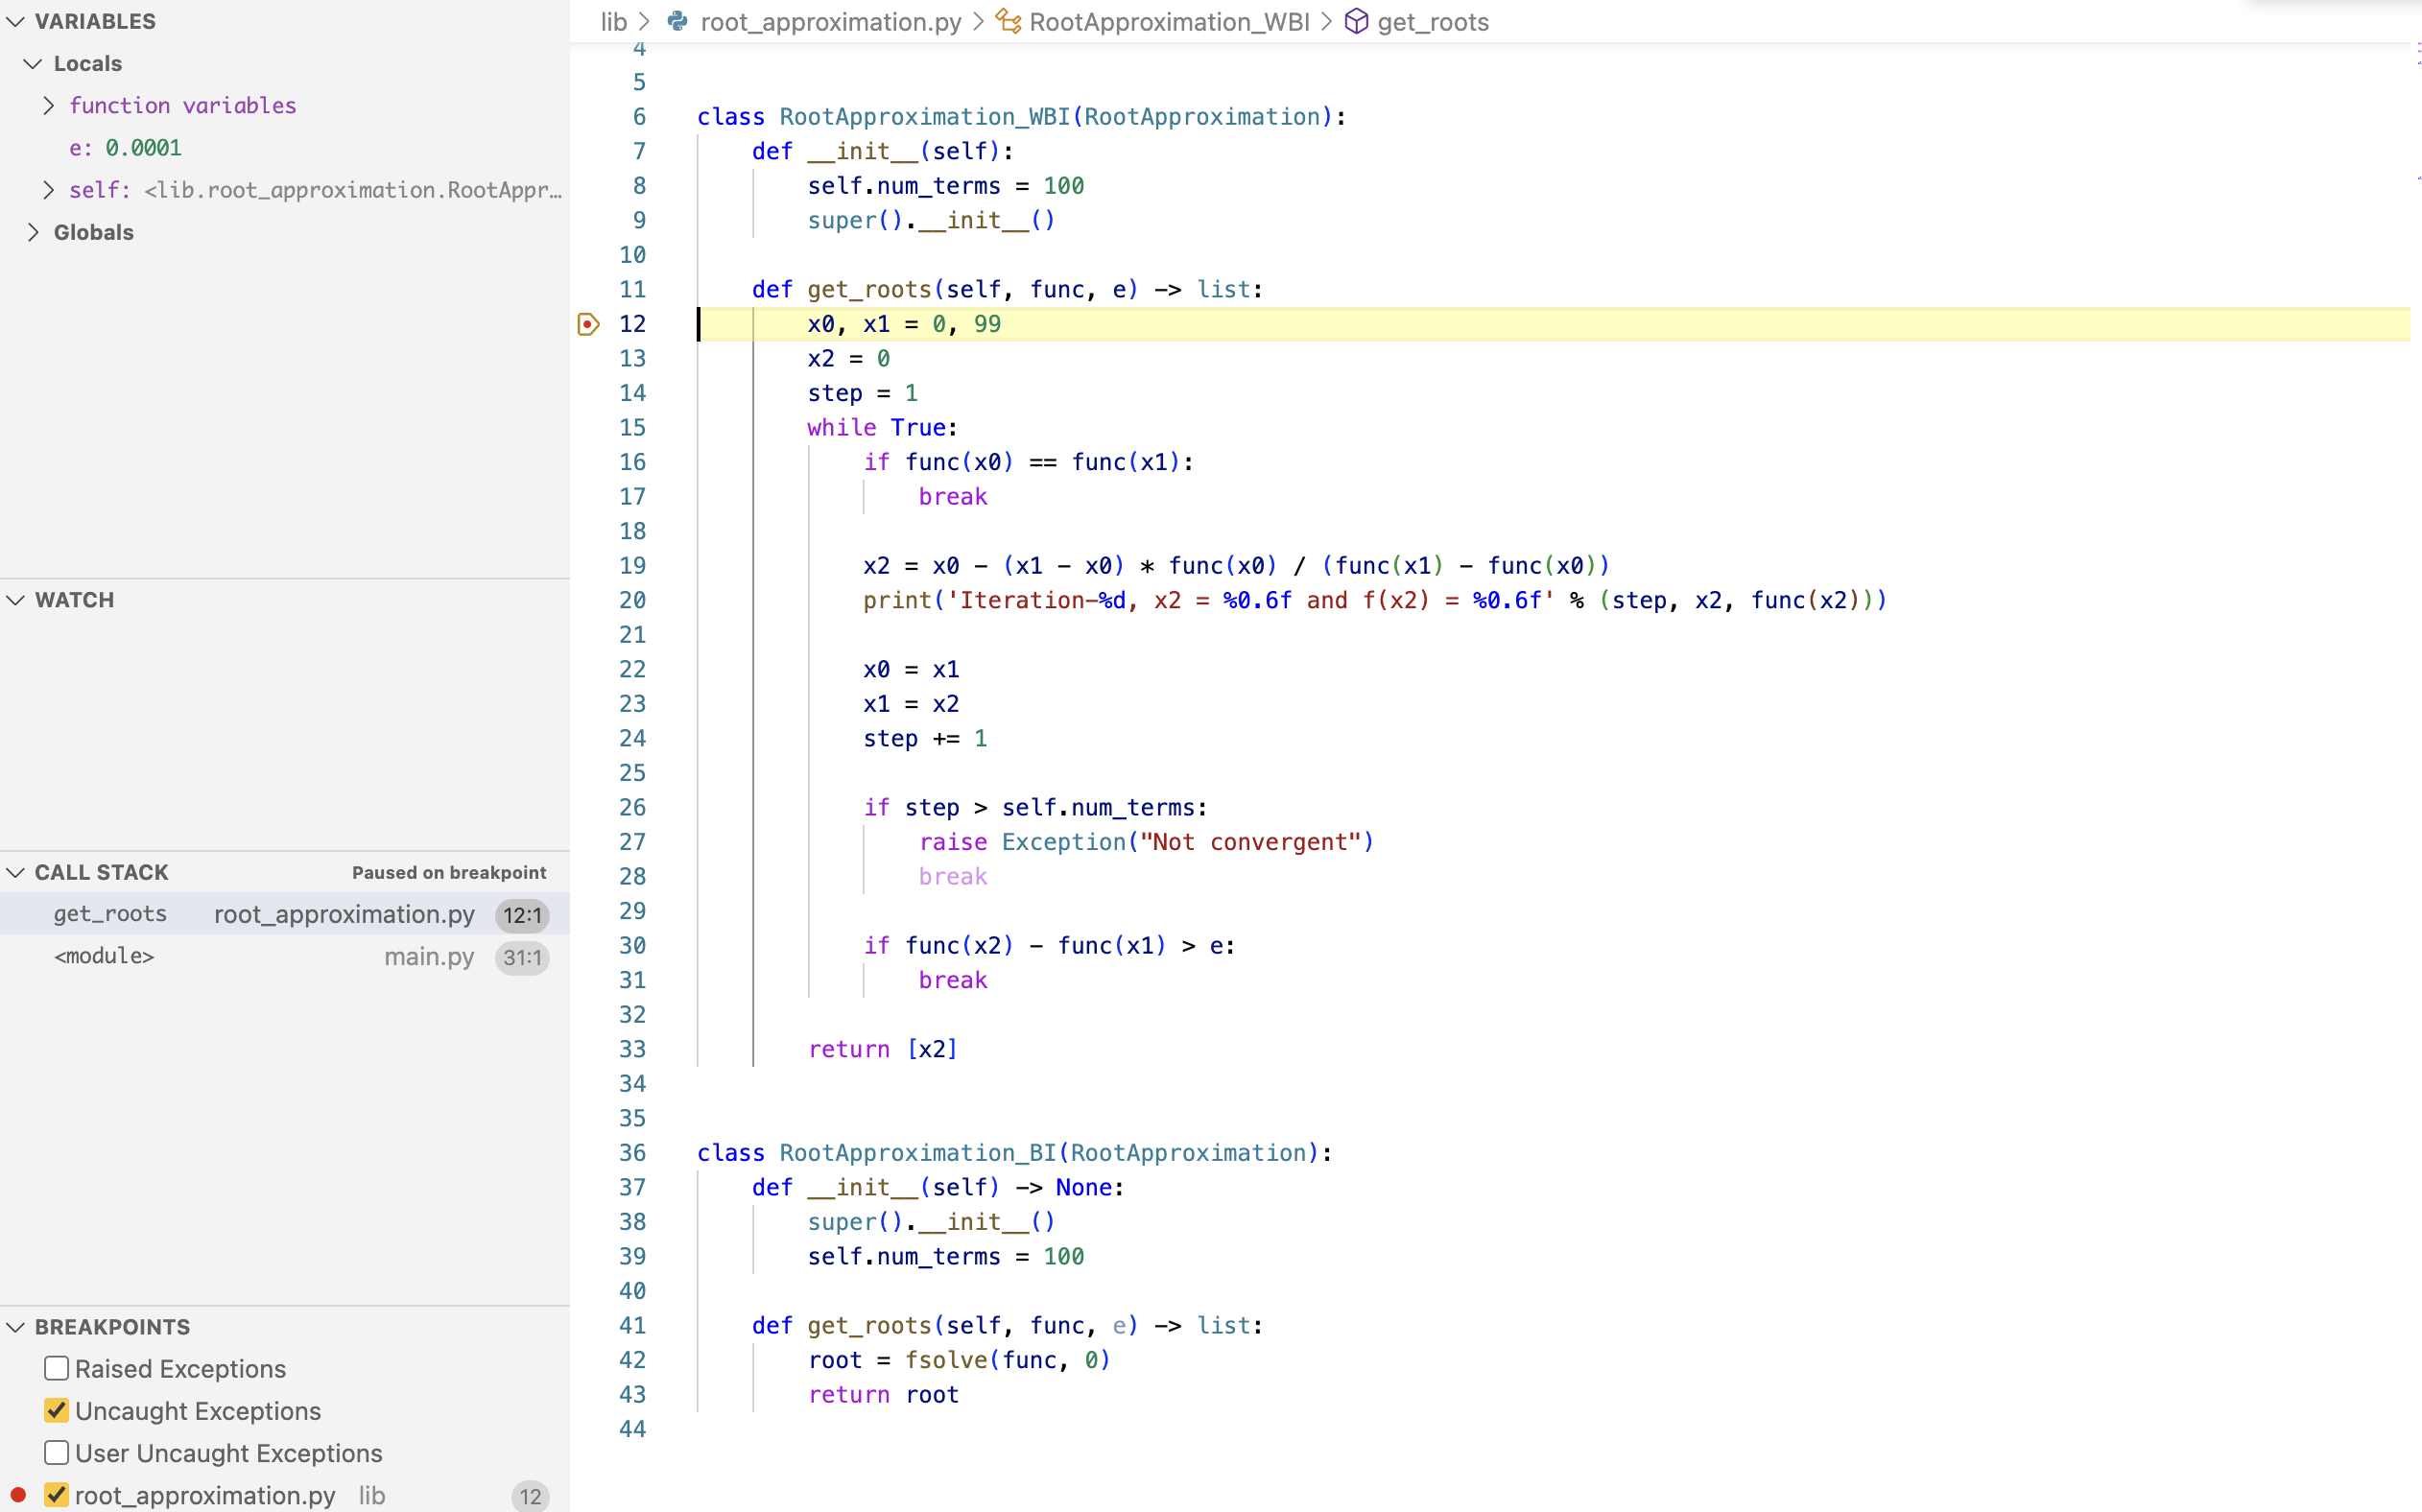
\includegraphics[scale= 0.3]{resources/debugger}}
      \caption{Debugger in action}
      \label{fig:Debugger}
    \end{figure}

  \section{Programming Style}
  Python Enhancement Proposals or PEPs are the documents that establish standards in the Python community. Most PEPs describe new features for Python or Python's standard library, but a few of them are more nebulous. PEP 8 is one of those\cite{python}. The guidelines provided under PEP 8 were followed during the development of the source code. The PyLint linter was used to enforce this. 

  \section{PyDoc}
    The PyDoc documentation system was used to document the source code
    \begin{figure}[h!]
      \centering
      \frame{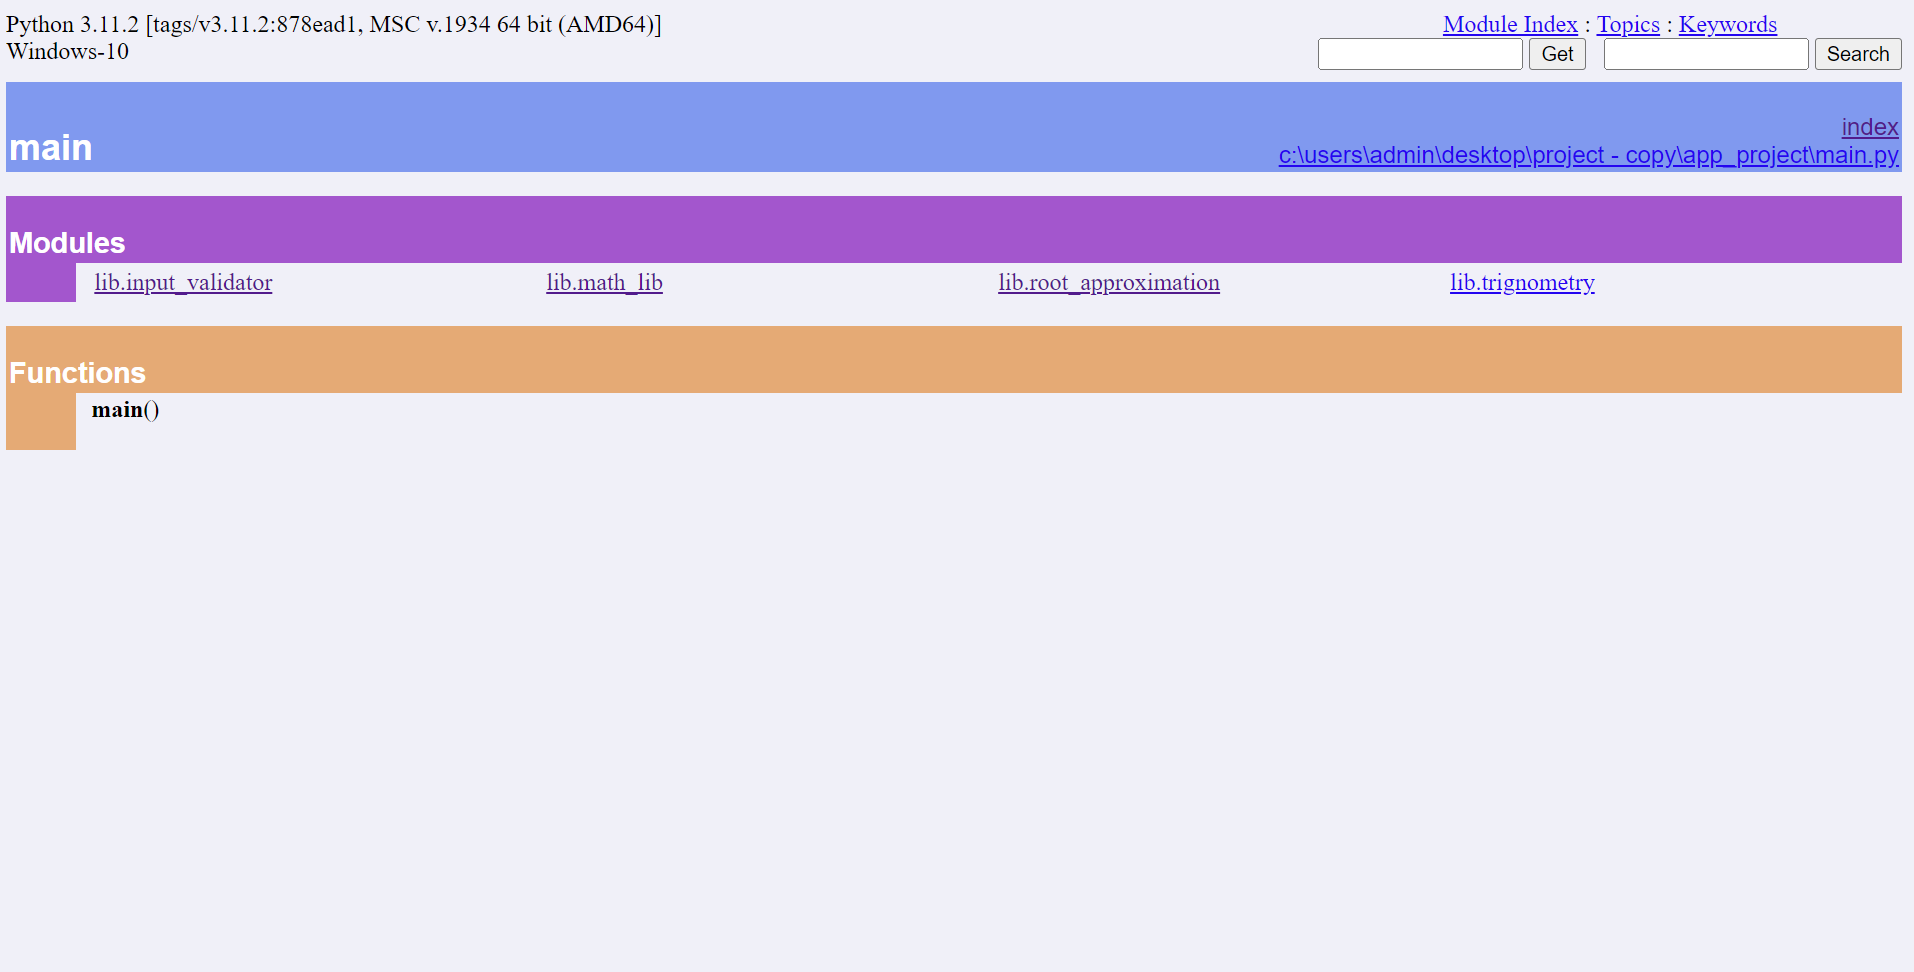
\includegraphics[scale= 0.4]{resources/pydoc.png}}
      \caption{Documentation using Pydoc}
      \label{fig:pydoc}
    \end{figure}


